\chapter{Capa de servicio}
\label{chapter:servicio}

En el capítulo anterior describimos la capa de \textit{streaming} de nuestro proyecto, este lo dedicaremos a la capa de servicio que se encargará de servir los datos procesados en la capa anterior a los usuarios.


\begin{figure}[!ht]
	\centering
	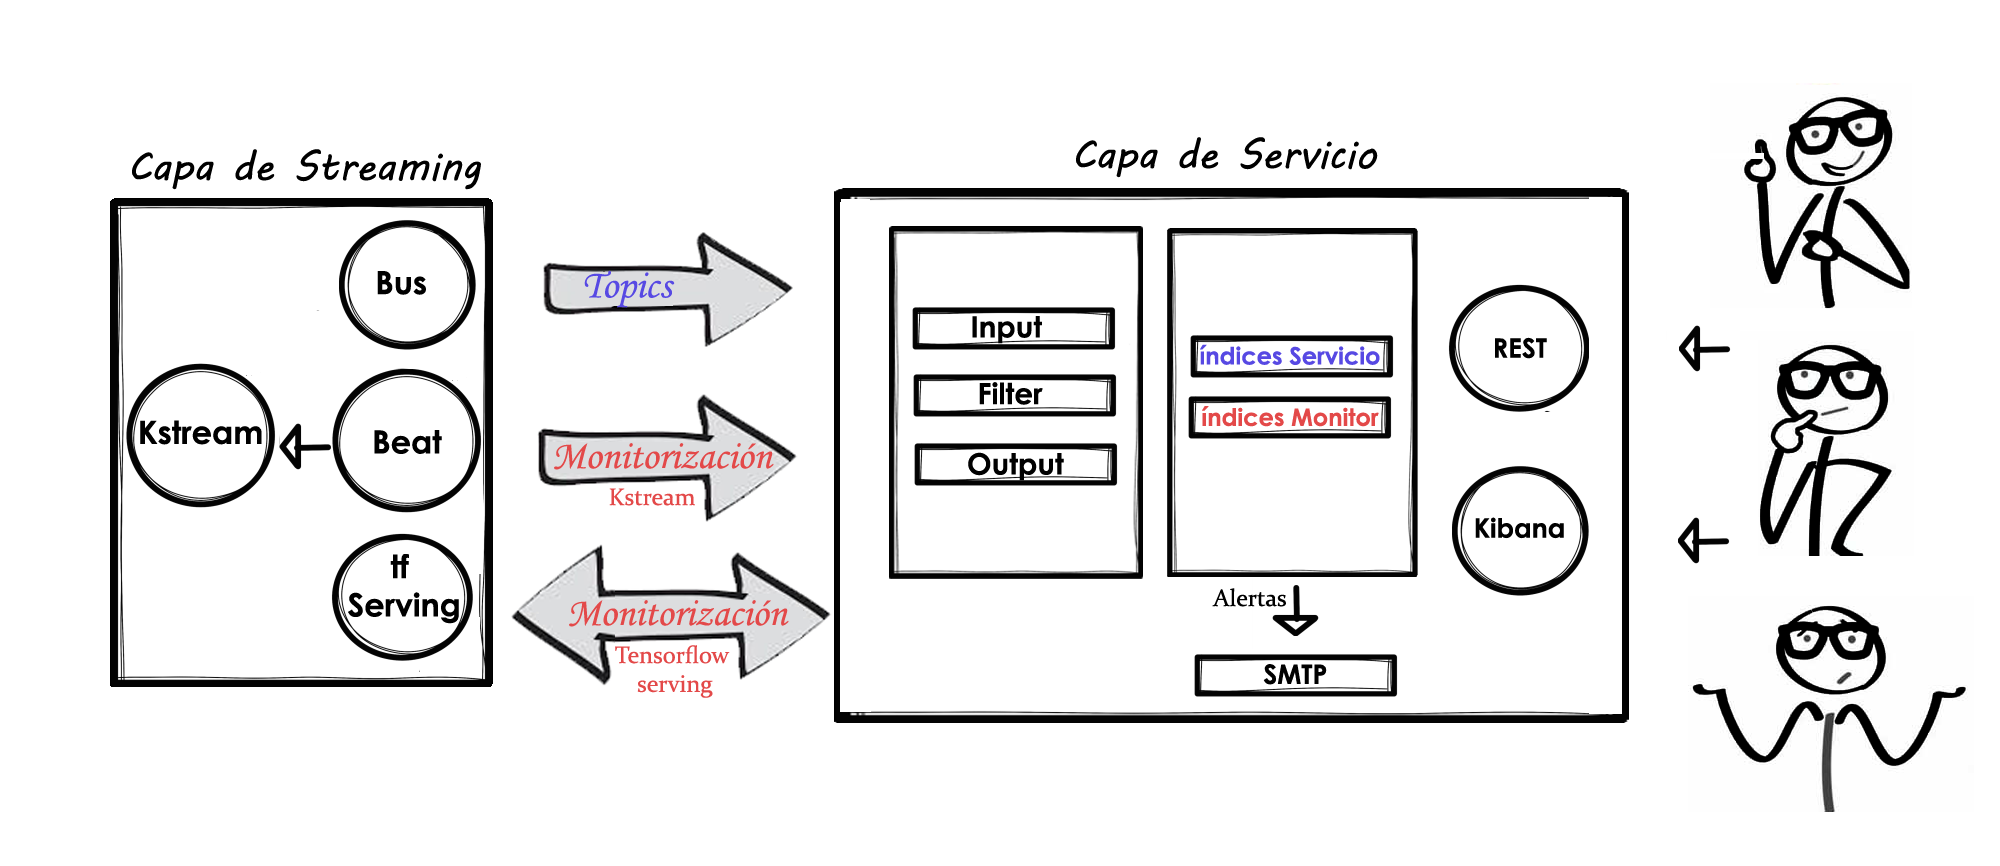
\includegraphics[width=1\textwidth]{images/serv/servicelayer_v1}
	\caption{Capa de servicio}
	\label{fig:servicelayer}
\end{figure}


En la figura \ref{fig:streamlayer} podemos ver un \textit{zoom} de la capa de servicio de nuestra arquitectura. Vemos que a esta capa nos llegan tanto los datos de monitorización, como los datos de servicio. En esta capa se hace un ligero procesado de los datos mediante Logstash, antes de insertarlos en Elasticsearch siguiendo un modelo predefinido de datos. Por último, la información almacenada puede generar alertas o puede ser consultada por los usuarios de diversas formas.

A lo largo del capítulo analizaremos en primer lugar cómo se realiza la carga de los datos, posteriormente veremos el modelado de los datos y los campos más relevantes, a continuación mostraremos algunas visualizaciones prediseñadas para que puedan ser consultadas por los usuarios y, por último, mostraremos las diferentes formas de realizar el alarmado.

El código y los ficheros de configuración al completo de todo lo que veremos en el capítulo puede encontrarse en \href{https://github.com/megmontero/topics-callcenter/tree/master/elk}{https://github.com/megmontero/topics-callcenter/tree/master/elk}.


\section{Ingesta de datos}
A lo largo de esta sección describiremos la forma en la que los datos se ingestan en la capa de servicio. El elemento principal de esta ingesta es \textbf{Logstash}, este componente es el encargado de llevar todos los datos, tanto del servicio como de monitorización a la capa de servicio mediante un \textit{\textbf{pipeline}}. 

Un \textit{pipeline} en Logstash describe el flujo que deben seguir los datos y se compone de tres fases: \textit{Input}, \textit{filter} y \textit{output}. Estas tres fases se corresponden con la extracción, transformación y carga de un proceso ETL tradicional. A lo largo de esta sección describiremos, usando el \textit{pipeline} desarrollado, cada una de las tres fases.


\subsection{\textit{Input}}

La fase \textit{input} es la encargada de la entrada de los datos, Logstash posee numerosos \textit{plugins} diferentes, los cuales pueden esperar pasivamente a recibir un evento escuchando en un puerto o ir al origen del evento de una forma activa.

A continuación mostramos el \textit{input} usado en nuestro proyecto.


\begin{minted}[
 	gobble=0,
 	frame=single,
 	linenos, 
 	fontsize=\footnotesize]{groovy}
input {
  beats {
    id => jmx_5010
    port => 5010
    client_inactivity_timeout => 86400
  }

  kafka {
        id => "topic_calls_topic"
        topics => ["TOPICS.CALLS"]
        sasl_jaas_config => "org.apache.kafka.common.security.scram.ScramLoginModule required username='topic_user'  password='topic_pwd';"
        security_protocol => "SASL_PLAINTEXT"
        sasl_mechanism => "SCRAM-SHA-256"
        client_id => "logstash"
        bootstrap_servers => "kfk1,kfk2,kfk3"
        codec => "json"
        group_id => "logstash"
        tags => ["kafka"]
        
    }


    http_poller {
        urls => {
            metrics => "http://tf-baja-model:8501/monitoring/metrics"
        }
        request_timeout => 60
        schedule => { "every" => "1m" }
        tags => ["tf"]
        codec => "plain"
  }


} 	
 	
\end{minted}

En el \textit{input} mostrado podemos ver los siguientes \textit{plugins} de entrada: 

\begin{itemize}
\item \textit{\textbf{Beats}} (línea 2): Este \textit{plugin} de entrada permanece escuchando en un puerto en espera de recibir eventos. Los eventos deben estar en el formato de los agentes \textit{beats} del \textit{stack} de Elastic. A través de esta entrada nos llegarán los datos de monitorización de los servicios de Kafka Streams. 

\item \textit{\textbf{Kafka}} (línea 11): Este \textit{plugin} permite que Logstash se conecte a un \textit{topic} de Apache Kafka y reciba de manera asíncrona todos los eventos del mismo. A través de esta entrada nos llegarán los eventos propios del servicio, con la clasificación de las llamadas.

\item \textbf{\textit{Http\_poller}} (línea 23): Este \textit{plugin} se diferencia con los demás en que va a preguntar a un API REST cada cierto tiempo, en lugar de recibir eventos. En este caso tenemos programado un intervalo de un minuto para cada consulta. En esta entrada recogeremos los eventos de monitorización de Tensorflow Serving.


\end{itemize}


\subsection{\textit{Filter}}

En la fase \textit{filter} se realizarán todas las transformaciones necesarias sobre los datos de entrada. En el siguiente código podemos ver la fase \textit{filter} de nuestro proyecto \textit{pipeline}. 

\begin{minted}[
 	gobble=0,
 	frame=single,
 	linenos, 
 	fontsize=\footnotesize]{groovy}
filter {
    if ("jmx" in [tags]){
        mutate{
            add_field => { "[period][ms]" => "%{[metricset][period]}" }
            split => ["[service][address]", ":"]
            add_field => { "service_short" => "%{[service][address][0]}" }
        }
        if ([jolokia][jolokia_metrics][uptime]){
            mutate{
                add_field => { "[uptime][ms]" => "%{[jolokia][jolokia_metrics][uptime]}"}
            }
        }
        if ([jolokia][jolokia_metrics][process-rate]){
            mutate{
                add_field => { "[process][rate]" => "%{[jolokia][jolokia_metrics][process-rate]}"}
                add_field => { "[process][latency][avg][ms]" => "%{[jolokia][jolokia_metrics][process-latency-avg]}"}
            }
            dissect {
                mapping => {
                    "[jolokia][jolokia_metrics][mbean]" => "%{}=%{kstream}-%{}-%{thread},%{}"
                }
            }
            if ([jolokia][jolokia_metrics][process-latency-max]){
                mutate{
                    add_field => { "[process][latency][max][ms]" => "%{[jolokia][jolokia_metrics][process-latency-max]}"}
                }
            }

        }
        mutate{
            remove_field => ["event", "host", "@version", "ecs", "metricset", "jolokia"] 
            rename => ["service_short", "service" ] 
        }

    }
    if ("tf" in [tags]){
        grok {
            match => { "message" => ":tensorflow:cc:saved_model:load_attempt_count{model_path=\"%{DATA}\"\,status=\"%{DATA:status}\"}" }
        }
        grok {
            match => { "message" => ":tensorflow:core:graph_run_time_usecs_histogram_sum{}\s%{NUMBER_SCI:tf_total_usecs}"}
            pattern_definitions => {"NUMBER_SCI" => "%{NUMBER}(e%{NUMBER})?"}

        }
        grok {
            match => { "message" => ":tensorflow:core:graph_run_time_usecs_histogram_count{}\s%{NUMBER_SCI:total_calls}"}
            pattern_definitions => {"NUMBER_SCI" => "%{NUMBER}(e%{NUMBER})?"}

        }  
        mutate{
            remove_field => ["message", "@version"] 
            convert => {
                "tf_total_usecs" => "float"
                "total_calls" => "integer"
                }
            add_field => { "service" => "tf-bajafactura" }
        }
        ruby {
                code => "event.set('[process][latency][avg][ms]', (event.get('tf_total_usecs') / (event.get('total_calls')) /1000).round)"
                remove_field => ["tf_total_usecs"]
        }
        mutate{
            rename => ["total_calls","[process][total]" ] 
        }
    }
    if ("kafka" in [tags]){        
            ruby {
                code => "hash = event.to_hash
                         hash.each do |k,v|
                                 if v == nil
                                         event.remove(k)
                                 end
                         end"
            }
    }
}
\end{minted}

Como podemos observar la fase \textit{filter} se divide en tres partes bien diferenciadas dependiendo de los tipos de eventos que hemos visto durante el \textit{input} . A continuación comentaremos brevemente cada una de estas partes: 

\begin{itemize}
\item \textbf{Eventos de \textit{beats}}:  Diferenciamos estos eventos por el \textit{tag} ``jmx'' que hemos introducido en ellos en el origen. Las transformaciones que realizamos sobre estos eventos tienen como objetivo adaptar los datos al formato que deseamos. Así vemos principalmente operaciones de renombrado, de \textit{dissect} o \textit{split} (que extraen partes de un campo)  y de borrado de campos que no nos interesan. 

\item \textbf{Eventos de \textit{http\_poller}}: Estos eventos contienen el \textit{tag} ``tf'' añadido en el \textit{\textit{input}}. Principalmente utilizamos el filtro \textit{grok} que nos ayuda a extraer mediante expresiones regulares las métricas que necesitamos para nuestra monitorización.

\item \textbf{Eventos de \textit{kafka}}: Estos eventos contienen el \textit{tag} ``kafka'' que nos ayuda a diferenciarlos del resto. Los datos ya viajan en \textit{Kafka} tal y como los necesitamos, por lo tanto, únicamente eliminamos  mediante código Ruby los elementos que lleguen con un valor nulo.


\end{itemize}



\subsection{\textit{Output}}

La última fase es el \textit{output} en el cual definimos cual será la salida de los eventos recibidos en el \textit{input} una vez transformados por la fase \textit{filter}.


\begin{minted}[
 	gobble=0,
 	frame=single,
 	linenos, fontsize=\footnotesize]{groovy}
 output {
 
     if ("jmx" in [tags] or "tf" in [tags]){
         elasticsearch{
         
             hosts => ["elasticsearch.host"]
             index => "inbi-topicmodel-monitoring-w.%{+YYYY.ww}"
             user => "${USER_LOGSTASH}"
             password => "${PASS_LOGSTASH}"
         }
     }
 
     if ("kafka" in [tags]){
     
         
         elasticsearch{
         
             hosts => ["elasticsearch.host"]
             index => "inbi-topicmodel-topics-w.%{+YYYY.ww}"
             user => "${USER_LOGSTASH}"
             password => "${PASS_LOGSTASH}"
         }
         
     }
     
 }	
 	
\end{minted}

En este caso podemos ver que todas las salidas tienen como destino un índice de Elasticsearch. En nuestro caso, vemos que tenemos dos índices diferentes, uno para los datos de monitorización (``inbi-topicmodel-monitoring-w.\%\{+YYYY.ww\}'') y otro para los datos propios del servicio (``inbi-topicmodel-topics-w.\%\{+YYYY.ww\}''). Podemos ver que estos índices poseen un patrón final que indica el año y la semana actual, esto nos ayudará a la hora de definir la retención de cada uno de los índices.

\section{Modelo de datos}

Como hemos visto anteriormente los datos anteriores se almacenan en dos índices diferentes según su funcionalidad: servicio y monitorización. En esta sección veremos el formato de ambos índices. 

Aunque el formato de los mismos puede definirse de manera dinámica en \textit{Elasticsearch} no es lo recomendable, lo ideal es definir un \textit{mapping} que indique el formato que debe tener cada índice y los tipos de campos. 


En la definición de los \textit{mappings} usaremos diferentes tipos de campos que describiremos brevemente: 

\begin{itemize}
\item Fecha: Los campos de tipo fecha nos permiten configurar el formato en el que nos llegarán (ISO 8601, \textit{epoch}, \textit{epoch ms}, etc.).
\item Texto: En este caso nos encontramos con dos campos de textos diferentes: 
\begin{itemize}
\item \textit{keyword}: Este campo de texto permite ordenaciones y agregaciones. Suele usarse cuando no es necesario realizar búsqueda libre por el mismo y, por tanto, no es necesario calcular el índice invertido. Por defecto, hemos establecido que estos campos no puedan ser mayores de 256 caracteres. 
 
\item \textit{text}: Este campo nos permite realizar búsquedas libres de texto, pero no podemos agregar u ordenar por el. En nuestro proyecto lo usaremos para realizar búsquedas en las llamadas o mensajes de error. También es posible agregarle filtros y analizadores que nos ayuden a realizar nuestras búsquedas.
\end{itemize}


\item Númericos: En este tipo de campos nos encontramos con \textit{integer}, \textit{float} y \textit{short}. Que son idénticos a los que pueden definirse en cualquier lenguaje de programación.
\end{itemize}


A continuación mostramos el \textit{mapping} definido para nuestro campo de monitorización. 

\begin{minted}[
 	gobble=0,
 	frame=single,
 	linenos, 
 	fontsize=\footnotesize]{json}

{
        "@timestamp" : {
          "type" : "date"
        },
        "agent" : {
          "properties" : {
            "ephemeral_id" : {
              "type" : "keyword",
              "ignore_above" : 256
            },
            "hostname" : {
              "type" : "keyword",
              "ignore_above" : 256
            },
            "id" : {
              "type" : "keyword",
              "ignore_above" : 256
            },
            "name" : {
              "type" : "keyword",
              "ignore_above" : 256
            },
            "type" : {
              "type" : "keyword",
              "ignore_above" : 256
            },
            "version" : {
              "type" : "keyword",
              "ignore_above" : 256
            }
          }
        },
        "error" : {
          "properties" : {
            "message" : {
              "type" : "text"
            }
          }
        },
        "kstream" : {
          "type" : "keyword",
          "ignore_above" : 256
        },
        "period" : {
          "properties" : {
            "ms" : {
              "type" : "integer"
            }
          }
        },
        "process" : {
          "properties" : {
            "latency" : {
              "properties" : {
                "avg" : {
                  "properties" : {
                    "ms" : {
                      "type" : "integer"
                    }
                  }
                },
                "max" : {
                  "properties" : {
                    "ms" : {
                      "type" : "integer"
                    }
                  }
                }
              }
            },
            "rate" : {
              "type" : "short"
            },
            "total" : {
              "type" : "integer"
            }
          }
        },
        "service" : {
          "type" : "keyword",
          "ignore_above" : 256
        },
        "status" : {
          "type" : "keyword",
          "ignore_above" : 256
        },
        "tags" : {
          "type" : "keyword",
          "ignore_above" : 256
        },
        "thread" : {
          "type" : "short"
        },
        "uptime" : {
          "properties" : {
            "ms" : {
              "type" : "integer"
            }
          }
        }
      }

\end{minted}

Una vez visto el \textit{mapping} describimos brevemente los campos definidos:

\begin{itemize}
\item \textbf{\textit{Agent}} (línea 5): Contiene información del agente encargado de realizar la monitorización (solo aplicable para Metricbeat).

\item \textbf{\textit{Error}} (línea 33): Campo de error que nos muestra posibles errores que puedan producirse. 

\item \textbf{\textit{KStream}} (línea 40): Nombre del proceso de KStreams .

\item \textbf{\textit{Period}} (línea 44): Periodo con el que se recogen los eventos.

 \item \textbf{\textit{Process}} (línea 51): Métricas del proceso (latencias y tasa de procesamiento). 
 
 \item \textbf{\textit{Service}} (línea 79): Servicio que estamos monitorizando. 


 \item \textbf{\textit{Status}} (línea 83): Estado del servicio.
 
  \item \textbf{\textit{Thread}} (línea 91): Thread del \textit{KStream} actual. De utilidad cuando escalemos.
  
   \item \textbf{\textit{Uptime}} (línea 94): Tiempo que lleva levantada la máquina virtual de Java.

\end{itemize}


A continuación mostramos el \textit{mapping} del índice con las predicciones. 

\begin{minted}[
 	gobble=0,
 	frame=single,
 	linenos]{json}

{
        "@timestamp" : {
          "type" : "date"
        },
        "@version" : {
          "type" : "keyword",
          "ignore_above" : 256
        },
        "call_text" : {
          "type" : "text"
        },
        "call_timestamp" : {
          "type" : "date",
          "format" : "epoch_second"
        },
        "co_province" : {
          "type" : "keyword",
          "ignore_above" : 256
        },
        "co_verint" : {
          "type" : "keyword",
          "ignore_above" : 256
        },
        "control_success" : {
          "type" : "boolean"
        },
        "control_type" : {
          "type" : "keyword",
          "ignore_above" : 256
        },
        "duration" : {
          "type" : "integer"
        },
        "error" : {
          "type" : "text",
          "fields" : {
            "keyword" : {
              "type" : "keyword",
              "ignore_above" : 256
            }
          }
        },
        "model" : {
          "type" : "keyword",
          "ignore_above" : 256
        },
        "pred_type" : {
          "type" : "keyword",
          "ignore_above" : 256
        },
        "predictions" : {
          "type" : "float"
        },
        "province" : {
          "type" : "keyword",
          "ignore_above" : 256
        },
        "tags" : {
          "type" : "keyword",
          "ignore_above" : 256
        }
      }
\end{minted}

En este caso los campos coinciden con los descritos en el capítulo \ref{chapter:prod} para el \textit{topic} de Apache Kafka \textit{TOPICS.CALLS}.

\section{Visualizaciones}
Aunque los usuarios más avanzados podrán atacar a la información definida de los índices directamente mediante la \textit{API REST} de Elasticsearch, se han definido una serie de visualizaciones y cuadros de mando que simplifiquen el acceso a la información y muestren a los usuarios los aspectos más relevantes. 

A lo largo de esta sección mostraremos algunos de ellos. En primer lugar veremos las monitorizaciones creadas para el servicio propiamente dicho y, posteriormente, veremos las visualizaciones definidas para realizar la monitorización del mismo.


\subsection{Servicio}

En la figura \ref{fig:cmserv} podemos ver el cuadro de mando que se ha diseñado para consumir los datos de la clasificación de llamadas realizadas.  

\begin{figure}[!ht]
	\centering
	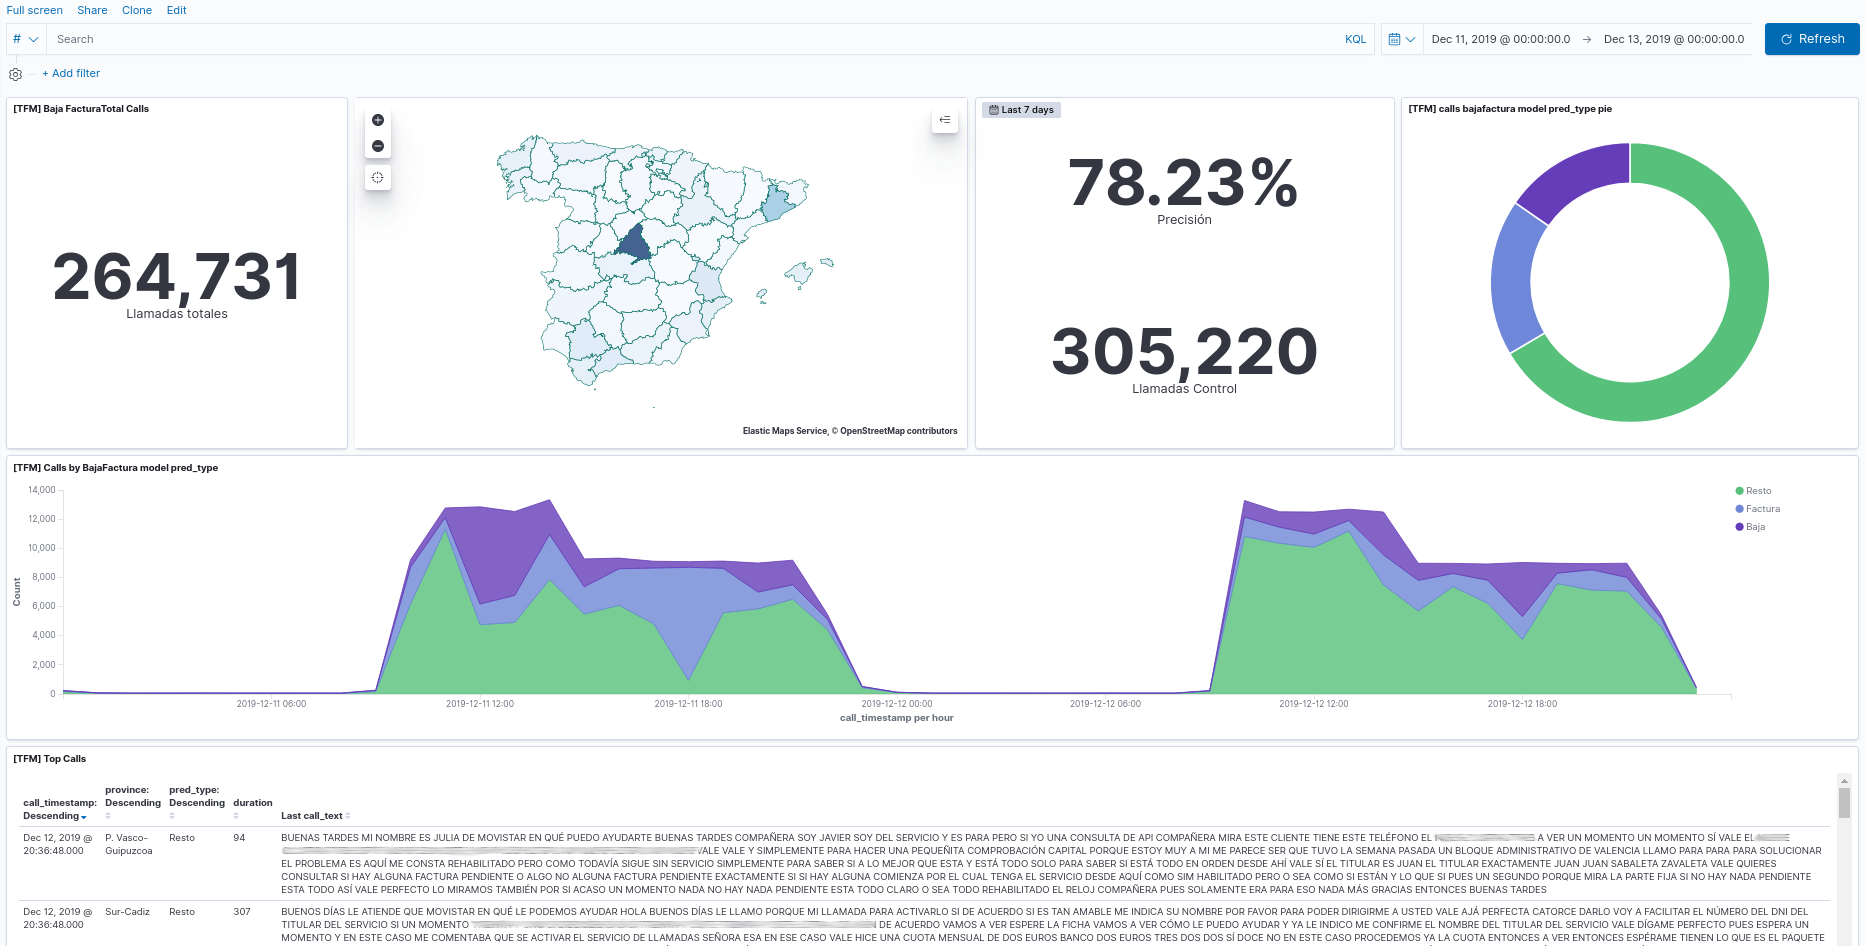
\includegraphics[width=1\textwidth]{images/serv/CM-calls}
	\caption{Cuadro de mando del servicio}
	\label{fig:cmserv}
\end{figure}


En este cuadro de mando podemos ver las siguientes visualizaciones: 

\begin{itemize}
\item \textbf{Llamadas Totales}: Situada en la parte superior izquierda muestra el número total de llamadas recibidas en el periodo determinado. En nuestro caso 2 días. 
\item \textbf{Mapa distribución de llamadas}: Muestra como se distribuyen las llamadas a lo largo de las provincias españolas. Vemos que las provincias con más concentración de llamadas son Madrid y Barcelona.

\item \textbf{Precisión últimos 7 días}: Muestra la precisión del modelo en los últimos 7 días y el número de llamadas de control que hemos recibido en ese periodo. Esto nos permitirá saber cómo de confiable es el modelo que se presenta.

\item \textbf{Distribución de llamadas}: Distribución de las llamadas en el intervalo seleccionado. Como se puede apreciar la mayoría de las llamadas pertenecen a la categoría ``Resto'' (como era de esperar). 

\item \textbf{Evolución de llamadas}: Vemos cómo evolucionan las llamadas a lo largo del tiempo. En nuestro caso al mostrar dos días podemos ver como la mayoría de la actividad se concentra en horario comercial.

\item \textbf{Top Calls}: Muestra para el periodo seleccionado las últimas llamadas recibidas junto a los datos de procedencia, duración y tipo predicho de la llamada.

\end{itemize}

El cuadro de mando mostrado se trata de un cuadro de mando dinámico en el que podemos filtrar por tiempo, tipo de llamada, provincia, etc. haciendo \textit{clicks} en cualquiera de las visualizaciones. 


\begin{figure}[!ht]
	\centering
	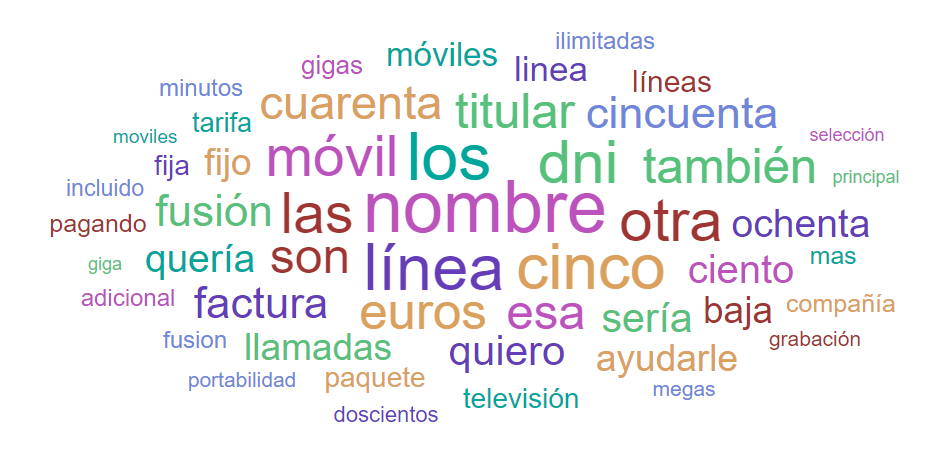
\includegraphics[width=0.8\textwidth]{images/serv/wordcloud}
	\caption{Nube de palabras desde la capa de servicio}
	\label{fig:wordcloud_kib}
\end{figure}


Además del cuadro de mando presentado, la capa de servicio con Kibana como frontal nos da una gran variedad de opciones para diseñar todo tipo de visualizaciones. Por ejemplo, como vemos en la figura \ref{fig:wordcloud_kib} sería posible la creación de una nueve de palabras con los términos más significativos directamente desde  esta capa. 

\subsection{Monitorización}
Al igual que tenemos un cuadro de mando para revisar el estado de servicio, hemos realizado uno para la monitorización del sistema, que nos permitirá estudiar el comportamiento del mismo.

\begin{figure}[!ht]
	\centering
	\includegraphics[width=1\textwidth]{images/serv/CM-monitoring}
	\caption{Cuadro de mando de monitorización}
	\label{fig:cmmon}
\end{figure}

En la figura \ref{fig:cmmon} observamos el cuadro de mando de monitorización compuesto por 4 visualizaciones diferentes: 

\begin{itemize}
\item \textbf{Procesos KStreams}: Es la visualización situada en la parte superior izquierda, muestra la tasa de procesamiento y  las latencias medias y máximas para cada proceso de KStreams a lo largo del tiempo. Las latencias medias de los procesos \textit{tokenizer} y \textit{sequencer} se sitúan en 1 ms, mientras que para el servicio \textit{predicter} esta en torno a los 150 ms. La tasa de procesamiento es la misma en todos los servicios, esto es lógico ya que por ellos pasa el mismo número de eventos.

\item \textbf{Proceso \textit{tf-bajafactura}}: Se trata de la visualización situada en la parte inferior izquierda, muestra la tasa de procesamiento y  la latencia media del proceso de \textit{tf-bajafactura}. Como vemos la latencia media es de unos 150 ms, lo que nos hace entender la latencia del servicio \textit{predicter}.
  
\item \textbf{Uso de Memoria}: Se muestra en la visualización situada en la parte superior derecha del cuadro de mando. Y muestra el total de memoria usado por todo el proyecto: Metricbeat, Logstash, servicios KStreams y Tensorflow Serving. Podemos ver que el total de la memoria usada es de unos 2GB. El grueso de la memoria está ocupado por Logstash (1GB) podríamos reducirlo, ya que es el tamaño inicial que le damos al \textit{Heap} de Java. 


\item \textbf{Uso de CPU}: En la parte inferior derecha mostramos el uso de \textit{CPU}. En este caso vemos que en todo momento estamos por debajo de los 2000 \textit{milicores} y que casi la totalidad de la CPU es usada por el servicio \textit{tf-bajafactura}. Esto es lógico debido a la gran cantidad de operaciones que es necesario realizar en la red neuronal. 

\end{itemize}


Para este cuadro de mando hemos utilizado los datos de métricas de consumo de la plataforma Openshift que ya se encontraban en Elasticsearch. Estos datos hacen referencia al consumo de CPU y memoria de los \textit{pods}. El resto de datos han sido ingestados específicamente para este proyecto, como hemos podido ver en el capítulo. 



\section{Alarmado}
Los cuadros de mando y visualizaciones definidos en el apartado anterior pueden ser de gran utilidad tanto para usuarios como para operadores de la plataforma, sin embargo nuestro objetivo no es pasarnos el día mirando cuadros de mando. Lo que pretendemos es disponer de un sistema de alertado que nos permita consultar la información en el momento que se produzca un evento determinado, para de este modo poder reaccionar según la necesidad. 

Se pueden definir una gran cantidad de alarmas que nos informen de diferentes eventos, pero en este apartado vamos a describir dos tipos diferentes que nos abrirán un abanico enorme de posibilidades: las alarmas estáticas y las alarmas dinámicas.

\subsection{Alarmas Estáticas}
Este tipo de alarmas definen unos umbrales fijos que en el caso de sobrepasarse provocan la realización de una acción. En nuestro proyecto, puede ser interesante para el equipo encargado de la explotación del sistema, establecer una serie de alarmas para controlar el uso de recursos de nuestros servicios. Esta tarea puede realizarse de una manera sencilla desde la propia capa de servicio con Elasticsearch.

Podemos ver un ejemplo de definición de alarma para controlar que la CPU no exceda de 3 \textit{cores} (3.000 \textit{milicores})  en el siguiente código: 


\begin{minted}[
 	gobble=0,
 	frame=single,
 	linenos, 
 	fontsize=\footnotesize]{groovy}
{
  "trigger": {
    "schedule": {
      "interval": "10m"
  } },
  "input": {
    "search": {
      "request": {
        "search_type": "query_then_fetch",
        "indices": [
          "ocp-metricbeat-*"
        ],
        "rest_total_hits_as_int": true,
        "body": {
          "size": 0,
          "query": {
            "bool": {
              "must": [
                {
                  "range": {
                    "@timestamp": {
                      "gte": "now-10m",
                      "lte": "now"
                } } },
                {
                  "term": {
                    "kubernetes.labels.app": {
                      "value": "tfm-mgm"
          } } ] } } },
          "aggs": {
            "total": {
              "sum_bucket": {
                "buckets_path": "servicio>cpu"
              }
            },
            "servicio": {
              "terms": {
                "field": "kubernetes.labels.service",
                "size": 100
              },
              "aggs": {
                "cpu": {
                  "max": {
                    "field": "kubernetes.pod.cpu.usage.nanocores",
                    "script": {
                      "inline": "(int) doc['kubernetes.pod.cpu.usage.nanocores'].value / 1000000",
                      "lang": "painless"
                    
  } } } } } } } } } },
  "condition": {
    "compare": {
      "ctx.payload.aggregations.total.value": {
        "gte": 3000
  } } },
  "actions": {
    "send_email": {
      "email": {
        "profile": "standard",
        "to": [
          "manuel.gomezmontero@telefonica.com"
        ],
        "subject": "[Topic-Model Alert] USO excesivo de CPU",
        "body": {
          "html": "El uso actual de CPU es de {{ctx.payload.aggregations.total.value}} milicores."
} } } } }	
 	
\end{minted}

Las alarma que hemos definido se compone de las siguientes fases: 
\begin{itemize}
\item \textit{\textbf{Trigger}} (línea 2): Cada cuanto se disparará la alarma. En nuestro caso cada 10 minutos.
\item \textit{\textbf{Input}} (línea 6): Entrada de la alarma. En nuestro caso una consulta DSL a Elasticsearch en la que obtenemos el uso total de CPU de los servicios del proyecto. 
\item \textit{\textbf{Condition}} (línea 50): Condición a verificar en la alarma. En nuestro caso número de \textit{milicores} mayor de 3.000.

\item \textit{\textbf{Actions}} (línea 55): Acción a realizar en el caso de que  la condición anterior se cumpla. En nuestro caso enviar un \textit{email} informando del uso actual.


\end{itemize}



\subsection{Alarmas mediante \textit{machine learning}}
Con la misma técnica anterior podríamos crear alarmas que comparen las métricas, en lugar de con un umbral, con lo ocurrido la semana o el día anterior. Sin embargo queremos ir más allá con este tipo de alarmas gracias a la funcionalidad de \textit{machine learning} de Elasticsearch. 

La funcionalidad de \textit{machine learning} de Elasticsearch nos permite crear modelos no supervisados que mediante distribuciones bayesianas detectan anomalías temporales. En nuestro caso lo utilizamos para crear un modelo que detecte anomalías en número de llamadas recibidas de cada tipo.  



\begin{figure}[!ht]
	\centering
	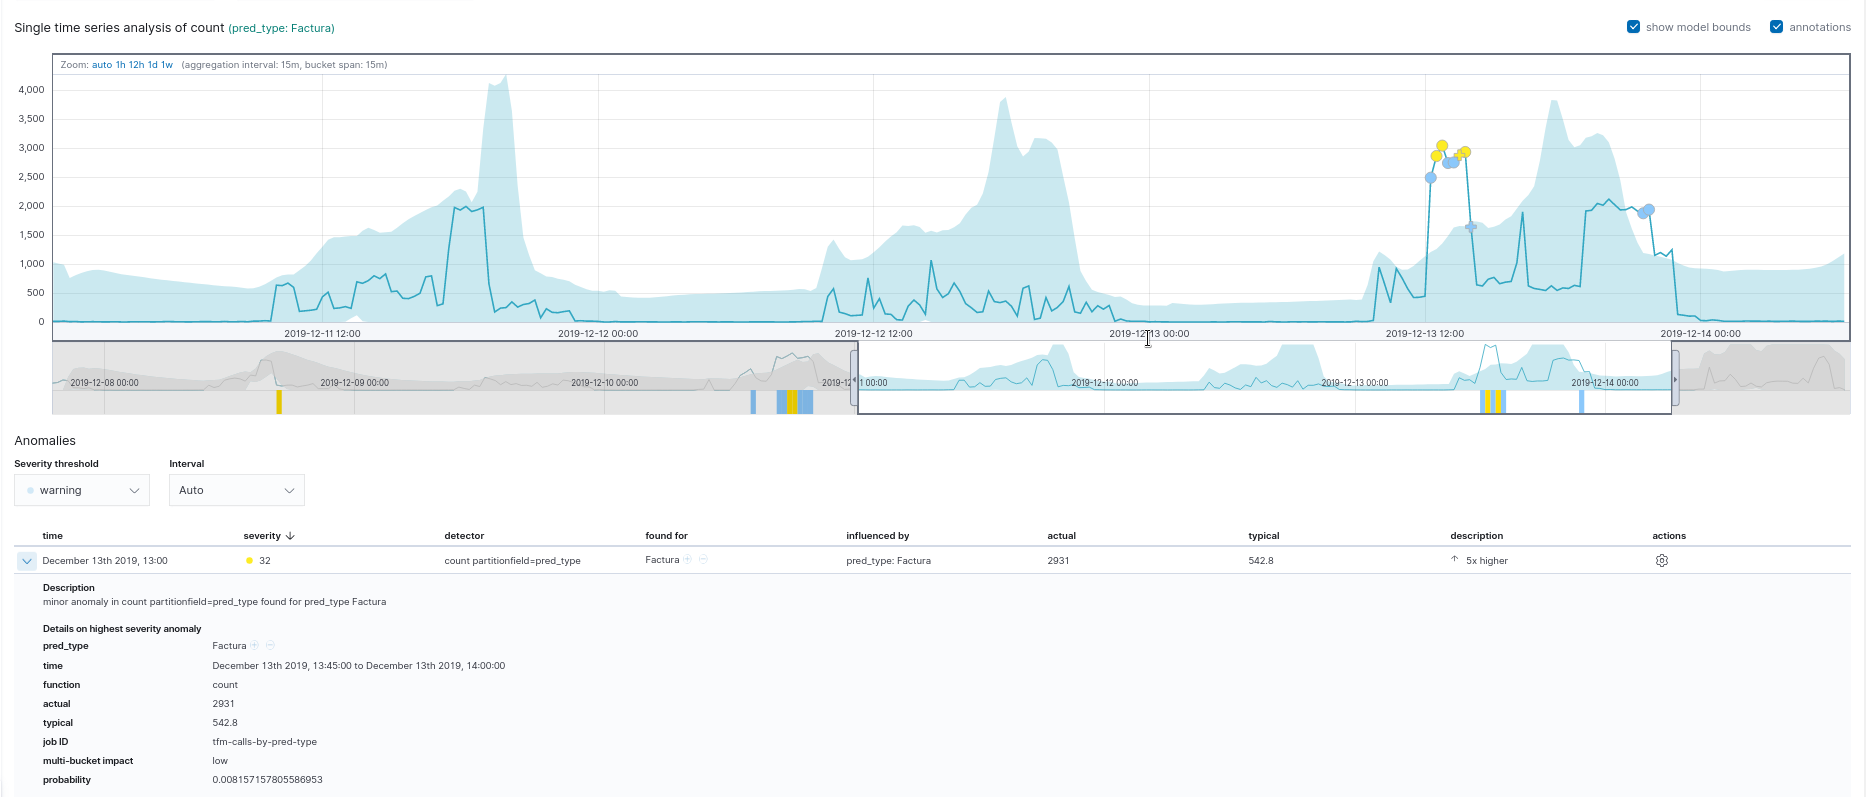
\includegraphics[width=1\textwidth]{images/serv/ml-factura}
	\caption{\textit{Machine learning}. Vista de métrica individual.}
	\label{fig:mlfactura}
\end{figure}

En la figura \ref{fig:mlfactura} podemos ver como funcionaría el modelo para el caso de las llamadas clasificadas como ``Factura''. La línea representa el número real de las llamadas recibidas de este tipo y la sombra va aprendiendo el comportamiento de este tipo de llamadas.  Aunque actualmente el histórico que tenemos de predicciones no es amplio, podemos ver como la sombra se va adaptando al horario comercial y en este caso vemos que las llamadas de este tipo se reciben más a últimas horas (puede deberse a no tener aún suficiente histórico o a un comportamiento habitual, pero es pronto para obtener conclusiones). Cuando una llamada sobrepasa ``la sombra'', el comportamiento esperado, consideramos que se ha producido una anomalía.  Estas anomalías tienen una severidad asociada, dependiendo de la probabilidad que existe de que esto ocurra. En la parte inferior de la figura \ref{fig:mlfactura} podemos ver una lista de estas anomalías con su severidad, el valor esperado y la probabilidad que el modelo tiene de que el valor actual pueda darse en situaciones normales.  


\begin{figure}[!ht]
	\centering
	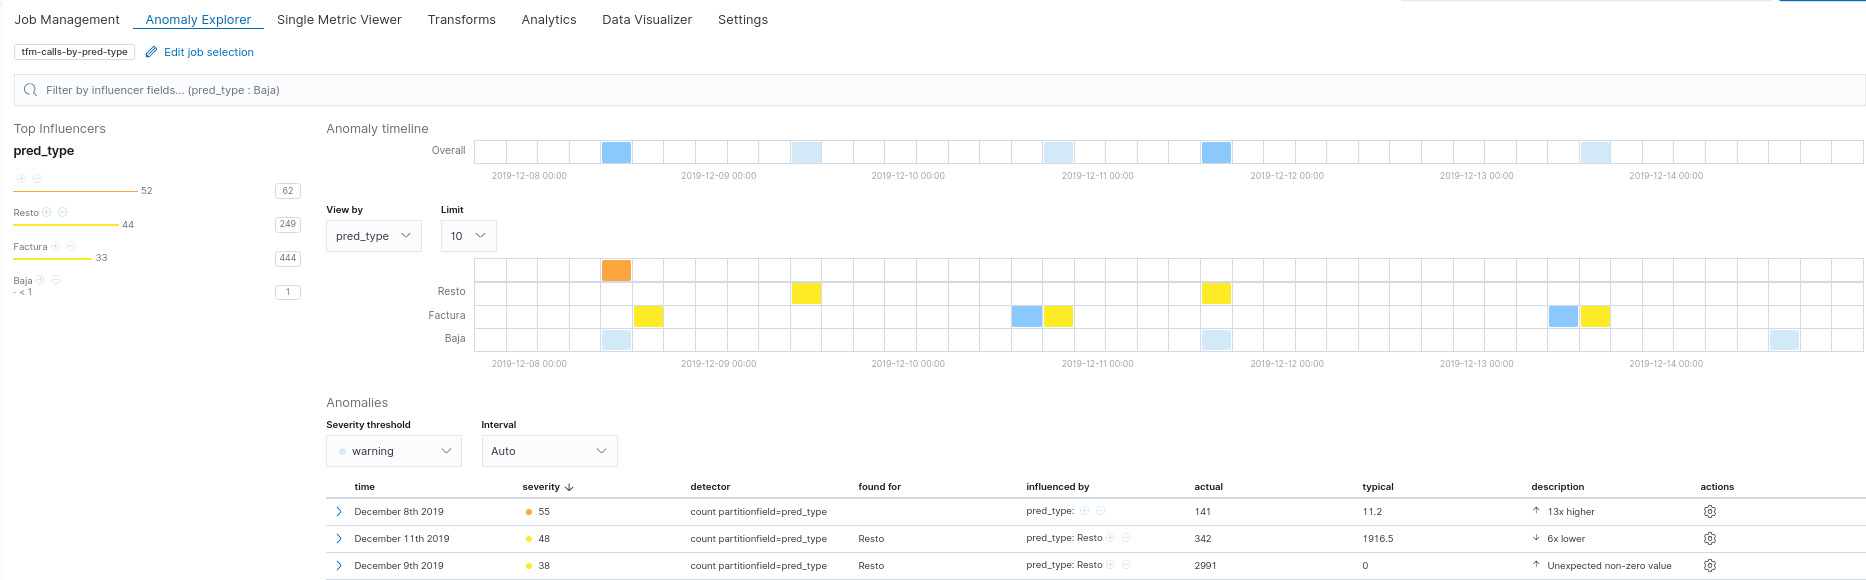
\includegraphics[width=1\textwidth]{images/serv/ml-total}
	\caption{\textit{Machine learning}. Vista de anomalías.}
	\label{fig:mlanom}
\end{figure}



Lo que hemos visto hasta ahora aplica a una métrica individual, el total de llamadas de la clase ``Factura'', sin embargo, como podemos ver en la figura \ref{fig:mlanom} se ha realizado tanto sobre el total de llamadas como sobre cada una de las clases de predicción del modelo. 

Esta detección de anomalías se realiza en tiempo real (más bien en \textit{batches} de pocos minutos), detectando anomalías en los datos conforme se van recibiendo. Las anomalías detectadas pueden utilizarse para crear una alarma al igual que en el apartado anterior ya que quedan almacenadas en un índice. 


La funcionalidad de crear alarmas con \textit{machine learning} es de gran utilidad en este caso de uso para, por ejemplo, en el caso de que se disparen las llamadas de ``Baja'' en un periodo no habitual, poder reaccionar en tiempo real y localizar la causa raíz. Esto no sería posible con alarmas estáticas y no tendría tanto potencial con alarmas que unicamente comparen, por ejemplo, con la semana anterior.





